\section{Shift Registers}
\label{sec:shift-registers}

A register capable of shifting the binary information held in each cell to its neighboring cell, in a selected direction, is called a \textit{shift register}. The logical configuration of a shift register consists of a chain of flip-flops in cascade, with the output of one flip-flop connected to the data input of the next flip-flop. All flip-flops receive common clock pulses, which activate the shift of data from one stage to the next.

The simplest possible shift register is one that uses only flip-flops, as shown in Fig. 3.
\begin{figure}[H]
  \centering
  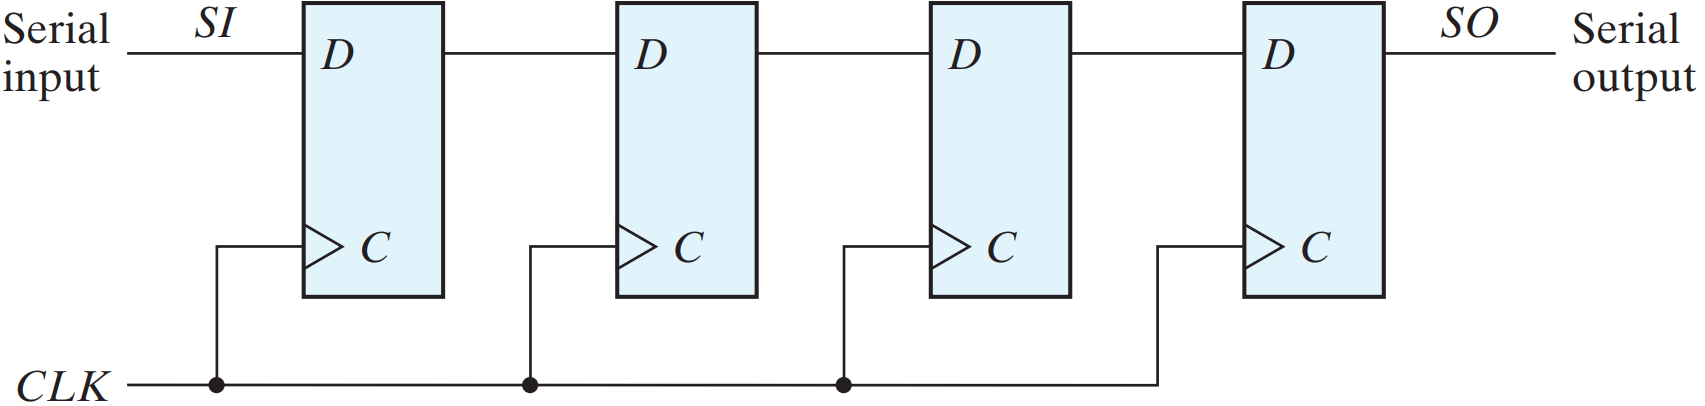
\includegraphics[width=\linewidth]{img/fig-6.3.png}
  \caption{Four-bit shift register}
  \label{fig:6.3}
\end{figure}
\noindent This shift register is unidirectional (left-to-right). Each clock pulse shifts the contents of the register one bit position to the right. The \textit{serial input} determines what goes into the leftmost flip-flop during the shift. The serial output is taken from the output of the rightmost flip-flop.

If the shift register of Fig. 3 is used, the shift can be controlled with an input by connecting the clock through an AND gate. This is not a preferred practice because it can lead to timing problems.


\subsection{Serial Transfer}
\label{subsec:serial-transfer}

The datapath of a digital system is said to operate in serial mode when \textit{information is transferred and manipulated one bit at a time}. Information is transferred one bit at a time by shifting the bits out of the source register and into the destination register. This type of transfer is in contrast to parallel transfer, whereby all the bits of the register are transferred at the same time.

The serial transfer of information from register $A$ to register $B$ is done with shift registers, as shown in the block diagram of Fig. 6.4(a). The shift control input determines when and how many times the registers are shifted. For illustration here, this is done with an AND gate that allows clock pulses to pass into the \textit{CLK} terminals only when the shift control is active. (This practice can be problematic because it may compromise the clock path of the circuit.)
\begin{figure}[H]
  \centering
  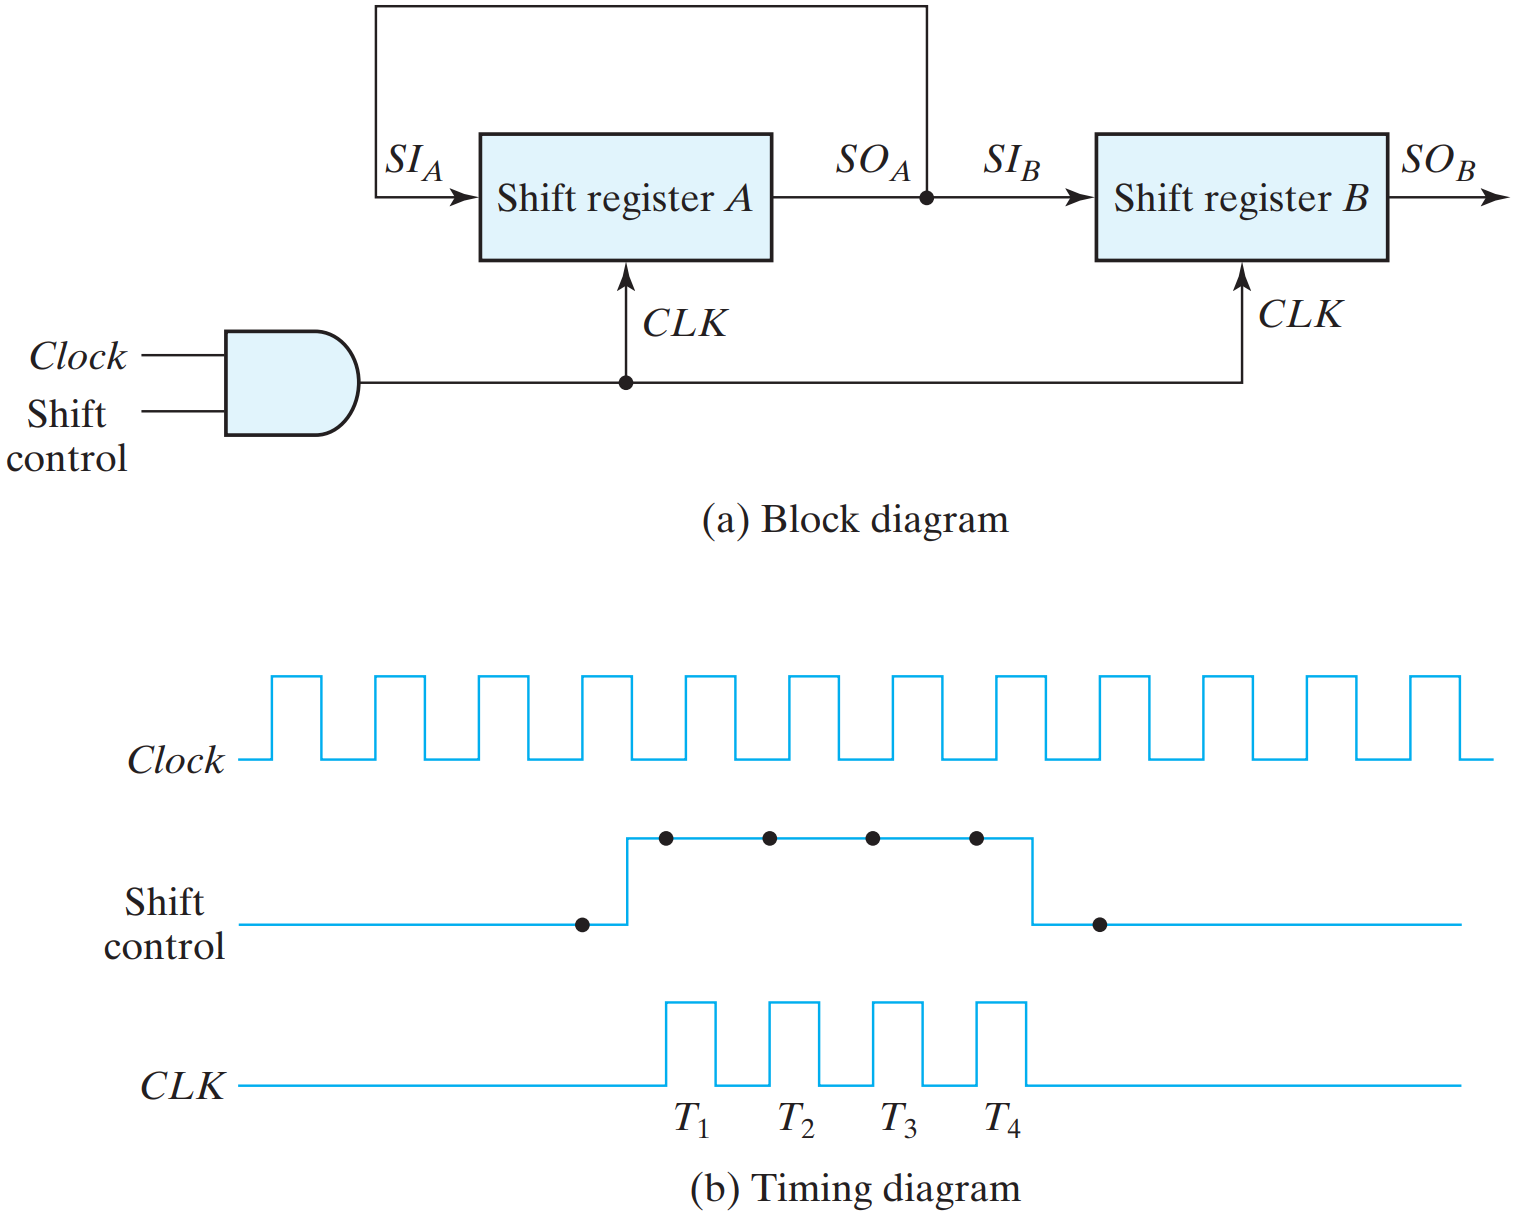
\includegraphics[width=\linewidth]{img/fig-6.4.png}
  \caption{Serial transfer from register $A$ to register $B$}
  \label{fig:6.4}
\end{figure}
\noindent The timing diagram is shown in the of Fig. 6.4(b). The shift control signal is synchronized with the clock and changes value just after the negative edge of the clock. The next four clock pulses find the shift control signal in the active state, so the output of the AND gate connected to the \textit{CLK} inputs produces four pulses: $T_1$, $T_2$, $T_3$, and $T_4$. Each rising edge of the pulse causes a shift in both registers. The fourth pulse changes the shift control to 0, and the shift registers are disabled.
\begin{figure}[H]
  \centering
  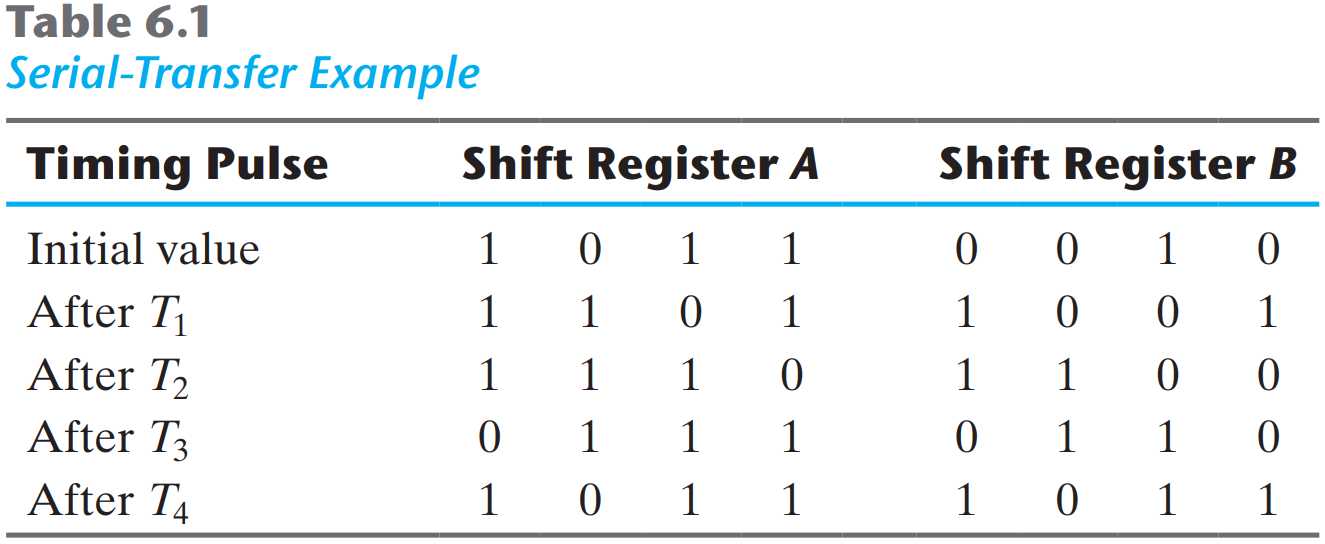
\includegraphics[width=\linewidth]{img/table-6.1.png}
  \label{table:6.1}
\end{figure}

One application of shift registers is converting between ``serial data'' and ``parallel data''. Computers typically work with multiple-bit quantities (ASCII: 8 bits long; Integers: 32 bits long.). But sometimes it's necessary to send or receive data serially, or one bit at a time. Some examples includes: Input devices such as keyboards and mice or output devices like printers.

To receive serial data using a shift register:
\begin{itemize}[leftmargin=0.7cm]
  \item The serial device is connected to the register's SI input.
  \item The shift register outputs Q3 - Q0 are connected to the computer.
  \item The serial device transmits one bit of data per clock cycle.
  \item These bits go into the SI input of the shift register.
  \item After four clock cycles, the shift register will hold a four-bit word.
  \item The computer then reads all four bits at once from the Q3-Q0 outputs.
\end{itemize}

\begin{figure}[H]
  \centering
  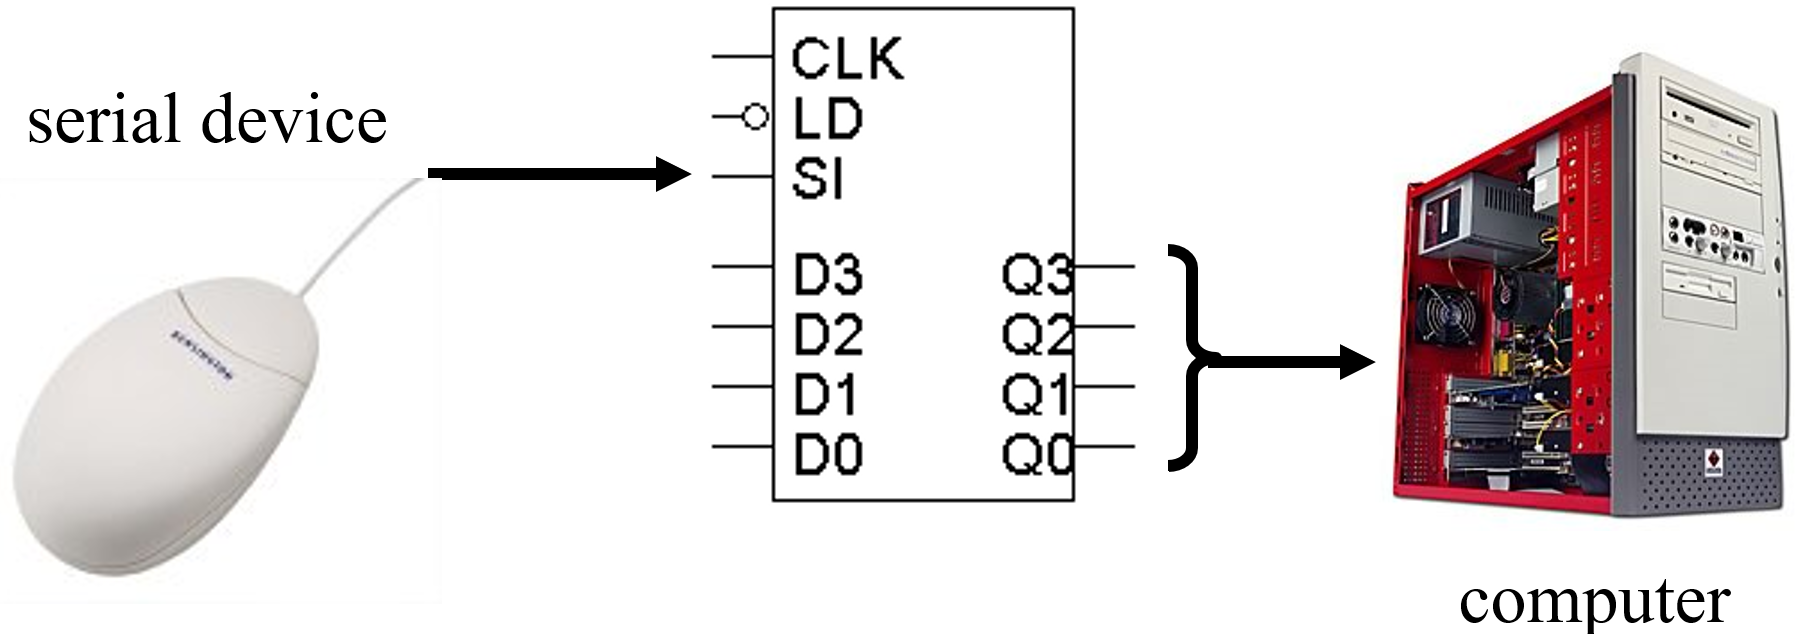
\includegraphics[width=\linewidth]{img/receiving-serial-data.png}
\end{figure}

To send data serially with a shift register, you do the opposite:
\begin{itemize}
  \item The CPU is connected to the register's D inputs.
  \item The shift output (Q3 in this case) is connected to the serial device.
  \item The computer first stores a four-bit word in the register, in one cycle.
  \item The serial device can then read the shift output.
  \item One bit appears on Q3 on each clock cycle.
  \item After four cycles, the entire four-bit word will have been sent.
\end{itemize}

\begin{figure}[H]
  \centering
  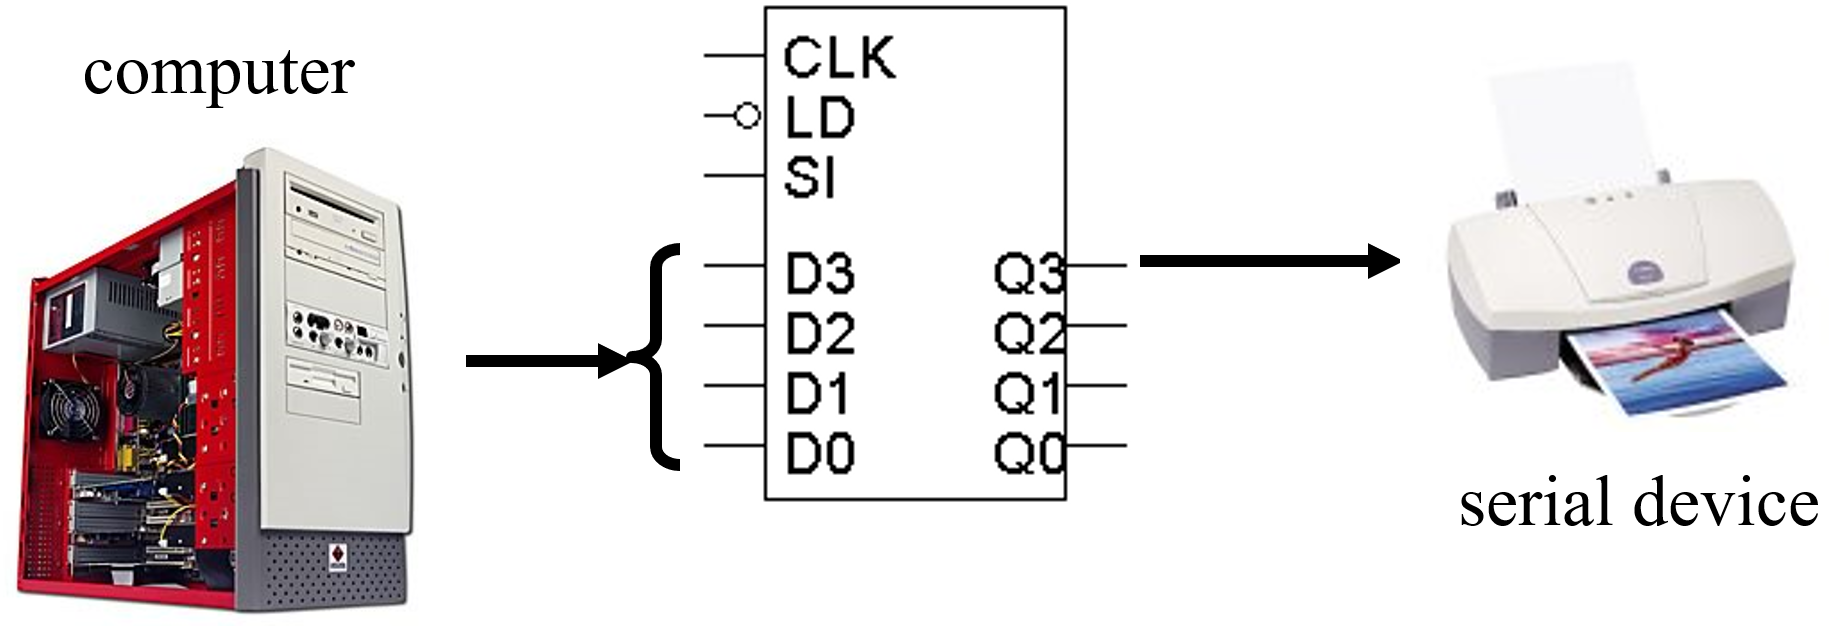
\includegraphics[width=\linewidth]{img/sending-data-serially.png}
\end{figure}


\subsection{Serial Addition}
\label{subsec:serial-addition}

Operations in digital computers are usually done in parallel because that is a faster mode of operation. Serial operations are slower because a datapath operation takes several clock cycles, but serial operations have the advantage of requiring fewer hardware components.

The two binary numbers to be added serially are stored in two shift registers. Beginning with the least significant pair of bits, the circuit adds one pair at a time through a single full-adder (FA) circuit, as shown in Fig. 5.
\begin{figure}[H]
  \centering
  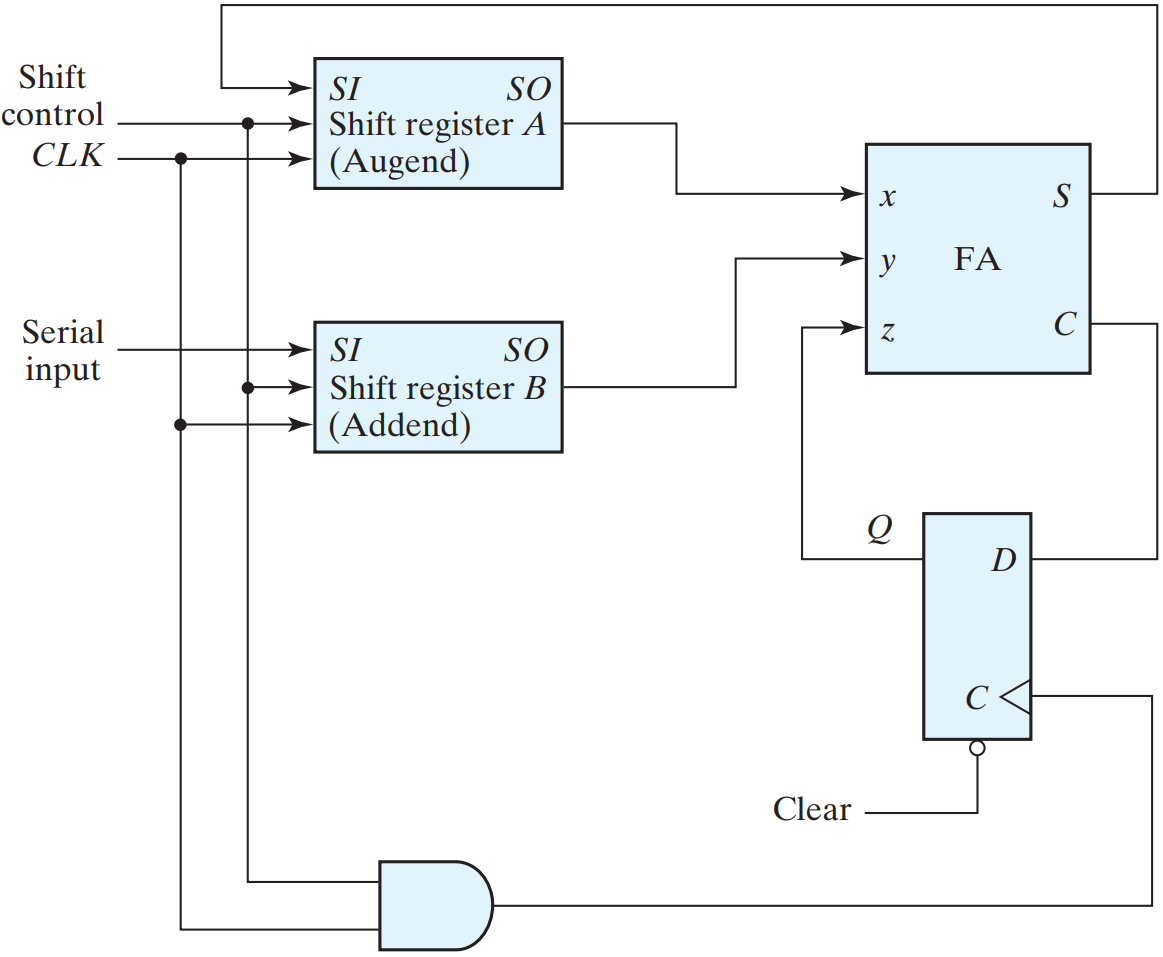
\includegraphics[width=\linewidth]{img/fig-6.5.png}
  \caption{Serial adder}
  \label{fig:6.5}
\end{figure}
\noindent Comparing the serial adder with the parallel adder, we note several differences.
\begin{itemize}
  \item The parallel adder uses registers with a parallel load, whereas the serial adder uses shift registers.
  \item The number of full-adder circuits in the parallel adder is equal to the number of bits in the binary numbers, whereas the serial adder requires only one full-adder circuit and a carry flip-flop.
  \item Excluding the registers, the parallel adder is a combinational circuit, whereas the serial adder is a sequential circuit, which consists of a full adder and a flip-flop that stores the output carry.
\end{itemize}
This design is typical in serial operations because the result of a bit-time operation may depend not only on the present inputs but also on previous inputs that must be stored in flip-flops.

To show that serial operations can be designed by means of sequential circuit procedure, we will redesign the serial adder with the use of a state table. First, we assume that two shift registers are available to store the binary numbers to be added serially. The serial outputs from the registers are designated by $x$ and $y$. The sequential circuit to be designed will not include the shift registers, but they will be inserted later to show the complete circuit. The sequential circuit proper has the two inputs, $x$ and $y$, that provide a pair of significant bits, an output $S$ that generates the sum bit, and flip-flop $Q$ for storing the carry. The state table that specifies the sequential circuit is listed in Table 6.2.
\vspace*{\fill}
\columnbreak
\begin{figure}[H]
  \centering
  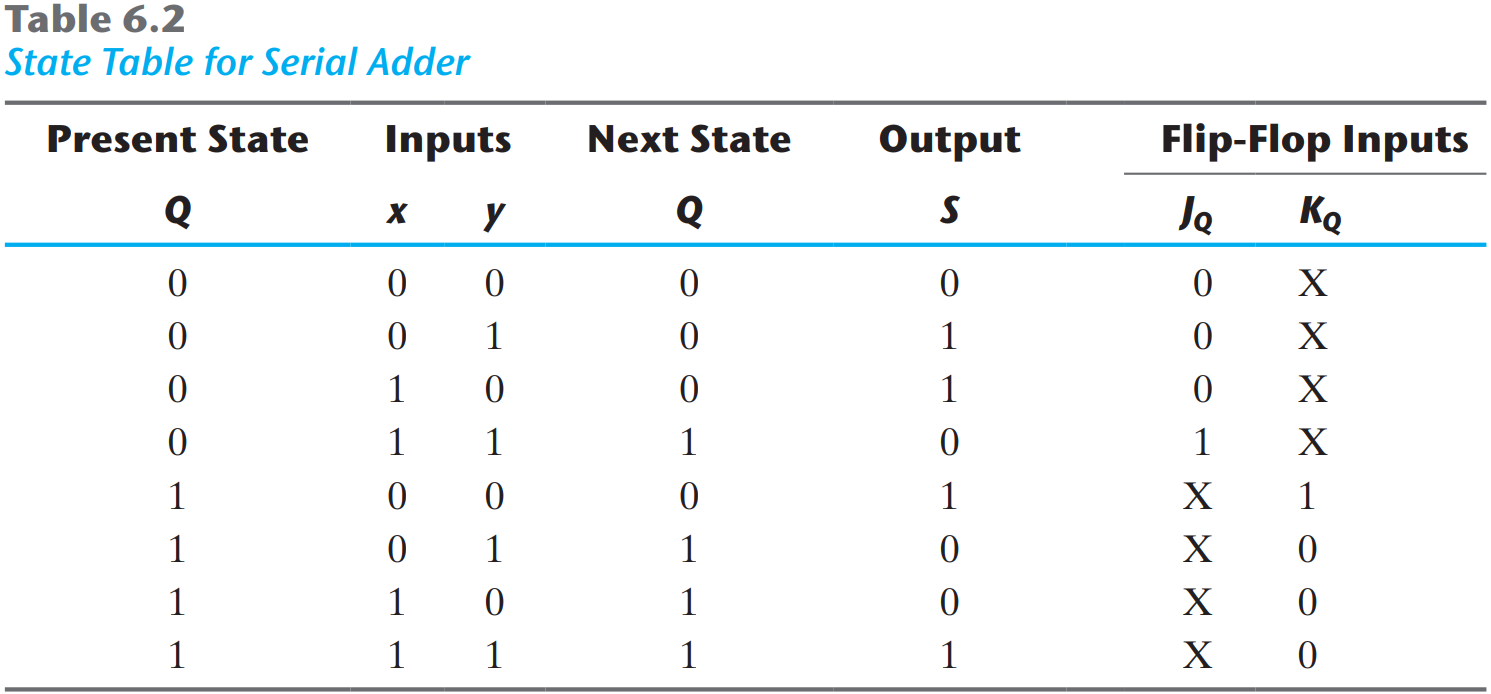
\includegraphics[width=\linewidth]{img/table-6.2.png}
  \label{table:6.2}
\end{figure}

If a $D$ flip-flop is used for holding $Q$, the circuit reduces to the one shown in Fig. 5. If a $JK$ flip-flop is used for $Q$, it is necessary to determine the values of inputs $J$ and $K$ by referring to the \textit{excitation table}. This is done in the last two columns of Table 6.2. The two flip-flop input equations and the output equation can be simplified by means of maps to
\begin{align*}
  J_Q &= xy\\
  K_Q &= x'y' = (x + y)'\\
  S &= x \oplus y \oplus Q
\end{align*}
The circuit diagram is shown in Fig. 6.6. The circuit consists of three gates and a $JK$ flip-flop. The two shift registers are included in the diagram to show the complete serial adder. Note that output $S$ is a function not only of $x$ and $y$, but also of the present state of $Q$. The next state of $Q$ is a function of the present state of $Q$ and of the values of $x$ and $y$ that come out of the serial outputs of the shift registers.
\begin{figure}[H]
  \centering
  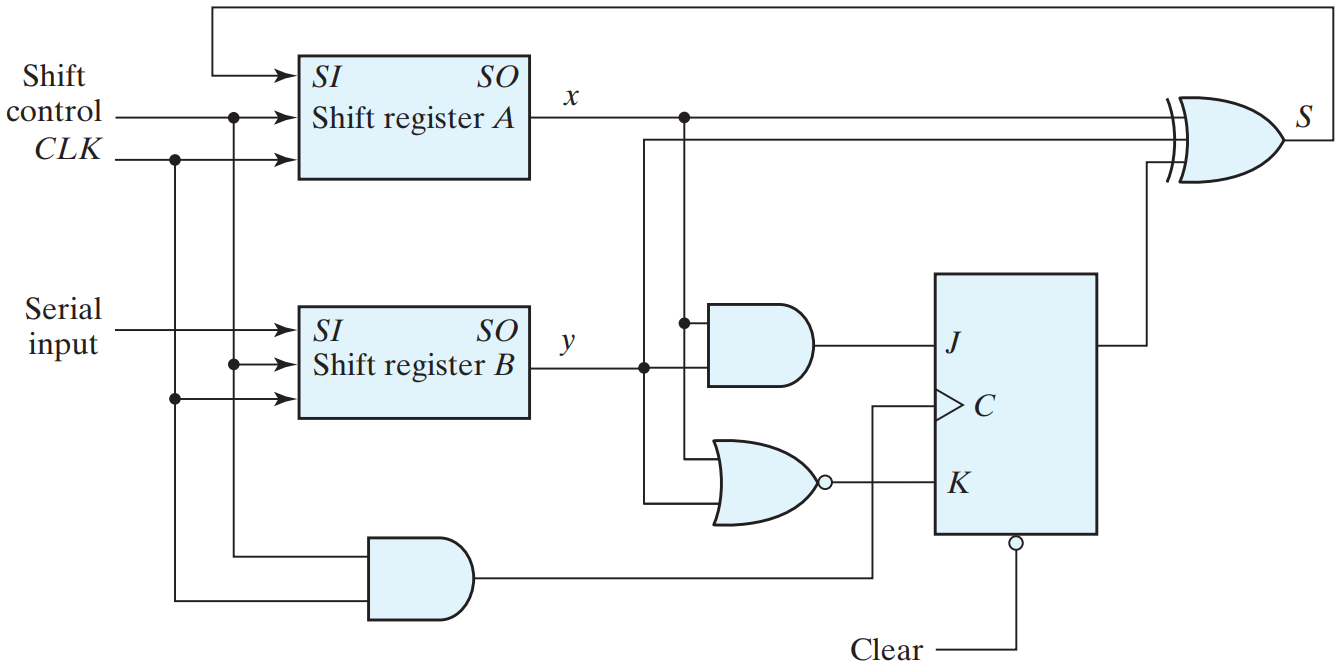
\includegraphics[width=\linewidth]{img/fig-6.6.png}
  \caption{Serial adder}
  \label{fig:6.6}
\end{figure}

\noindent\rule{\linewidth}{1pt}

\begin{figure}[H]
  \centering
  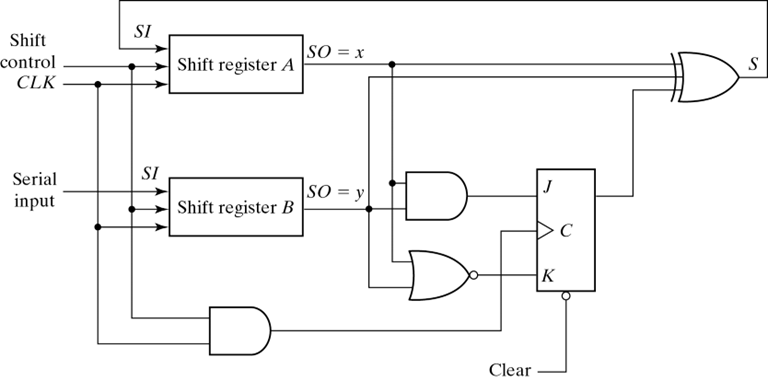
\includegraphics[width=\linewidth]{img/serial-adder-with-JK-FF.png}
  \caption*{Serial Adder with $JK$ Flip-Flop}
  \label{fig:serial-adder-with-jk-ff}
\end{figure}

\begin{practice}{Practice Exercise 6.2}
Explain why a serial adder is a sequential circuit.\\

\textbf{Answer:} The circuit uses a flip-flop.
\end{practice}

\subsection{Universal Shift Register}
\label{subsec:universal-shift-register}

If the flip-flop outputs of a shift register are accessible, then information entered serially by shifting can be taken out in parallel from the outputs of the flip-flops. If a parallel load capability is added to a shift register, then data entered in parallel can be taken out in serial fashion by shifting the data stored in the register.

Some shift registers provide the necessary input and output terminals for parallel transfer. They may also have both shift-right and shift-left capabilities. The most general shift register has the following capabilities:
\begin{enumerate}[leftmargin=0.7cm]
  \item A \textit{clear} control to clear the register to 0.
  \item A \textit{clock} input to synchronize the operations.
  \item A \textit{shift-right} control to enable the shift-right operation and the \textit{serial input} and \textit{output lines} associated with the shift right.
  \item A \textit{shift-left} control to enable the shift-left operation and the \textit{serial input} and \textit{output lines} associated with the shift left.
  \item A \textit{parallel-load} control to enable a parallel transfer and the $n$ input lines associated with the parallel transfer.
  \item $n$ parallel output lines.
  \item A control state that leaves the information in the register unchanged in response to the clock.
\end{enumerate}

If the register can shift in both directions and has parallel-load capabilities, it is referred to as a \textit{universal shift register}.

The block diagram symbol and the circuit diagram of a four-bit universal shift register that has all the capabilities just listed are shown in Fig. 7. The circuit consists of four $D$ flip-flops and four multiplexers. The four multiplexers have two common selection inputs $s_1$ and $s_0$.

\begin{figure}[H]
  \centering
  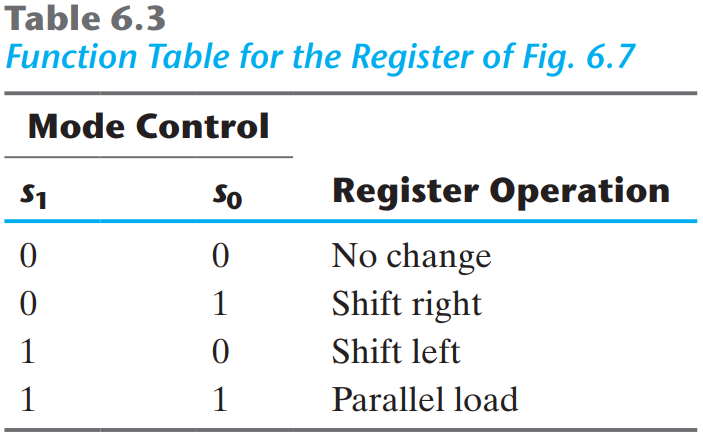
\includegraphics[width=\linewidth]{img/table-6.3.png}
  \label{table:6.3}
\end{figure}

\end{multicols}

\begin{figure}[H]
  \centering
  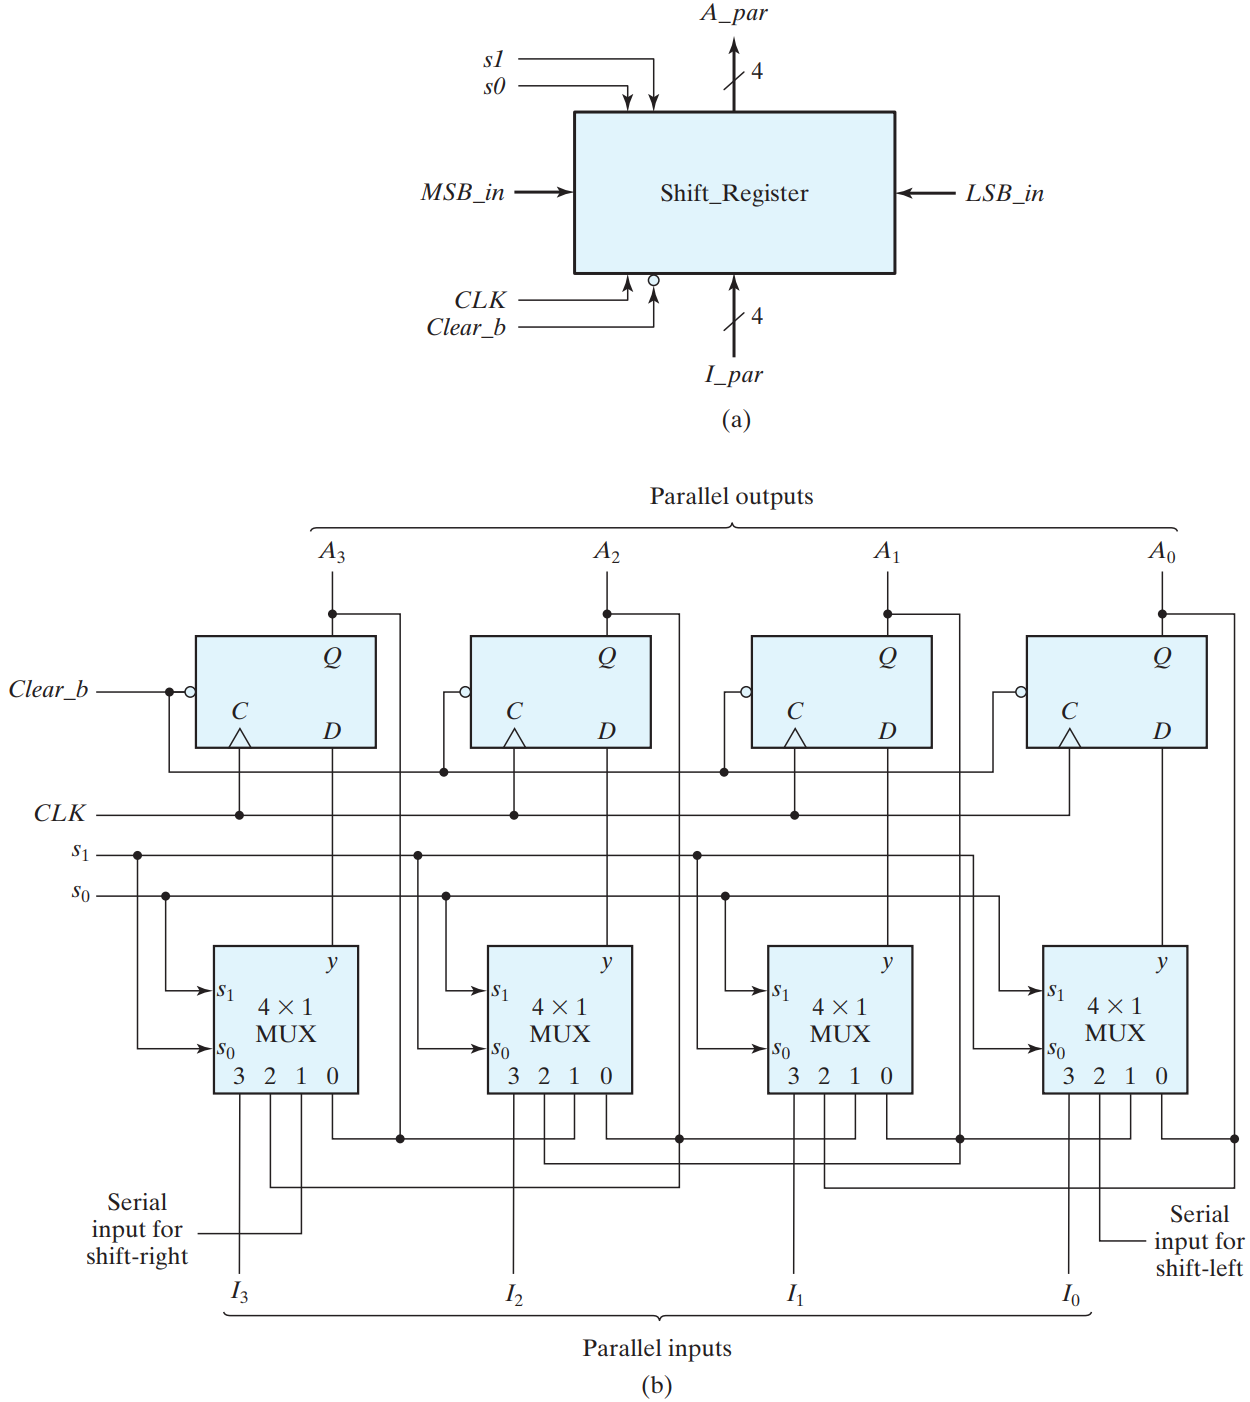
\includegraphics[width=\linewidth]{img/fig-6.7.png}
  \caption{Four-bit universal shift register}
  \label{fig:6.7}
\end{figure}


\begin{multicols}{2}
\setlength{\columnsep}{1.5cm}
\setlength{\columnseprule}{0.2pt}